\chapter{Daronpon: Datacenter Load Balancing Across Racks}
\label{chap:daronpon}

%\def\checkmark{\tikz\fill[scale=0.4](0,.35) -- (.25,0) -- (1,.7) -- (.25,.15) -- cycle;}
\newcommand{\toolname}{Daronpon}
\newcommand{\systemname}{Daronpon}

\section{Introduction}
\label{sec:intro}

To improve both performance and fault tolerance, datacenter
applications are provisioned to scale horizontally, with replicated
instances frequently spread across multiple racks of servers.  These
replicas must be carefully managed to meet strict service-level
objectives (SLOs) for both throughput and
latency~\cite{killer_microseconds,tail_at_scale}. These requirements
have birthed an architectural paradigm of highly replicated
microservices that can (nearly) arbitrarily fan out to deliver
ever-higher throughput, and whose functionality is scoped to provide
microsecond-timescale responses with low latency even in the tail.

Realizing this design pattern in practice poses multiple engineering
challenges, however.  Microsecond-timescale services must be resilient
to low-level system and network perturbations and short-lived
congestion events to achieve consistent
performance~\cite{facebook_microburst}.  These events arise within the
operating system, runtime, and application software as well as due to
network-level incast events, where a large number of clients send to a
common destination server, causing in-network buffering and
substantial queuing delays~\cite{facebook_memcache}.  Moreover, the
potential impact of these so-called ``microbursts'' increases with
network bandwidth.  Large bursts can lead to packet drops and
necessitate end-to-end retransmissions.

Experience shows that a responsive and effective load-balancing
strategy is key to managing overall service latency.  Given the
ultra-low service times of many modern datacenter services, end-to-end
approaches driven by the clients and servers themselves are unlikely
to meet demands, as many component service (i.e., computation) times
are smaller than datacenter-wide network latencies. Instead, we focus
on in-network load balancing techniques carried out by network
switches or middle boxes---often generally referred to as
``dispatchers''.  Recent work has shown the benefits of load balancing
with a server rack, for example R2P2~\cite{r2p2} and
Racksched~\cite{racksched}.  These approaches take into account server
load balancing, building upon prior approaches to core scheduling in
individual servers~\cite{IX,shinjuku,shenango,seda}. Further,
Vargaftik et al.~\cite{lsq} show that, for the multiple-dispatcher
environments that we target, a stable and highly efficient load
balancing approach is possible through a carefully controlled exchange
of status updates between servers and dispatchers.

We present \toolname, an inter-rack load balancer targeted to network
services with sub-RTT service times.  \toolname\ periodically
exchanges service-load information between dispatchers, either through
explicit gossip messages or piggybacked onto redirected application
requests.  We employ a logarithmic thresholding approach to minimize
the network overhead of state-exchange messages while ensuring that
application requests are forwarded to replicas with good performance.
Our system decreases the 99th-percentile tail latency by up to a
factor of two over random replica selection across a variety of
application workloads, enables scaling across heterogeneous server
configurations, and provides performance gains for service times as
low as two microseconds.

\section{Background}
\label{sec:background}

%\textbf{Data Center Replication:}

Modern datacenter applications are
replicated~\cite{rocksdb,memcached,mongodb} to provide fault
tolerance, scalability and flexible response to load
fluctuations. Often, individual application components are replicated
on the order of three times for fault tolerance. In the case of
sharding for scalability, however, the number of replicas can be many
orders of magnitude higher and even grow
dynamically~\cite{facebook_shard,google_slicer,microsoft_service_fabric}
as needed to service demand.

\subsection{Datacenter load balancing}
%%
Traditional application or ``layer-4'' load balancers operate across
the set of back-end services and maintain connection consistency for
long-lived flows. They are generally implemented in software using
commodity servers~\cite{cheetah, maglev, beamer, ananta}, although
some have explored using switches with hardware support~\cite{duet,
  silkroad}.  While effective at responding to end-host-driven load
imbalances, they are ill-positioned to address transient
variations in service times.

Conversely, conventional layer-3 load-balancing techniques focus on
dispersing traffic load in the network, and do not address server
imbalance.  For example, equal-cost multi-path routing (ECMP) load
balances flows using a hash of their 5-tuple. ECMP is widely deployed
due to the benefits it gains from average-case statistical
multiplexing.  It is well known, however, to cause load imbalance due
to hash collisions and when links fail.  A variety of improvements to
ECMP have been proposed, many using the concept of
flowlets~\cite{conga, clove, HULA, letitflow}: a group of packets
within the same flow separated from others by a large enough time
interval. Other schemes load balance per
packet~\cite{drill,flowbender,hermes}. Each of these in-network
techniques are complementary to our work, as they load balance
exclusively based on the state of the network and not the end-host
applications.

\subsection{Microsecond timescales}

Despite practitioners' attempts to spread demand evenly across both
servers and network fabrics~\cite{facebook:sigcomm15}, a certain
degree of variability is inevitable.  Indeed, as links speeds of 100 and
400-Gbps become the norm, hosts and switches can experience
significant traffic bursts over short periods of time. These bursts,
while lasting only a few microseconds, can cause congestion, lead to
increased jitter, and result in packet
drops~\cite{facebook_microburst}. As a concrete example, a switch with
64~MB of packet memory will overflow in 1.9~ms at
100~Gbps~\cite{tofino2} under incast scenarios.  While these events
originate in the network, the effect of that queuing cascades at the
application. Congestion impacts performance directly as batches of
requests are delivered in very short time periods.  Existing
end-to-end techniques struggle to react to microbursts effectively as
the durations of the microbursts are shorter than the network RTT
which bounds the response time of any end-host approach.

%\emph{Rack-scale load balancing:}

\toolname\ targets microsecond-timescale services which
do not involve long-lived connections.
%Maintaining connections for
%microsecond timescale load balancing wastes precious resource on
%switches. \toolname\ is
(We support any request/response service on top of a connection-less
transport or one with migration ability~\cite{crab,quic}.)  Techniques
for dispatching such microsecond-duration requests within an end-host
operating system have been explored recently~\cite{IX, shinjuku, snap,
  shenango, zygos}.  These end-host-based approaches use load-aware
schedulers to direct requests to CPU cores and to quickly rebalance
those allocations.  Extensions to these techniques demonstrate similar
scheduling performance at the scope of a entire server
racks~\cite{r2p2, racksched}. These efforts make use of programmable
switches to track end-host load at the rate of millions of requests
per second~\cite{tofino2}. Both R2P2~\cite{r2p2} and
Racksched~\cite{racksched} are confined to services which operate
entirely within a single rack due to a single control point within the
ToR switch. This limits the applicability of these schemes for the
majority of replicated applications which are distributed throughout
the datacenter.

Researchers have also explored explicitly integrating different
replication techniques with programmable switching hardware to avoid
RTT delays, including chain replication~\cite{netchain},
Raft~\cite{hovercraft}, and Paxos~\cite{nopaxos}.  In-network
replication techniques have also been proposed to alleviate
read/write conflicts~\cite{harmonia} and
contention~\cite{pegasus}. \toolname\ operates under the assumption
that replicas are interchangeable for all requests; our
techniques could be extended to support distributed protocols, however
\toolname\ would require protocol specific information.

\section{Challenges}
\label{sec:challenges}

Theoretically, optimal load balancing is attainable with centralized
algorithms~\cite{jsq_fcfs} that maintain full knowledge of the global
instantaneous system load.  A proven-optimal algorithm,
join-the-shortest-queue (JSQ), ensures requests experience minimal
queuing delay.  Unfortunately, centralization prevents cross-rack
sharding and scale-out designs.  In contrast, fully decentralized
approaches (e.g. client-based power-of-two designs~\cite{power_of_2})
require network-wide message round trips to measure load. As the
service time of requests approaches that of an RTT, the cost of
probing increases the latency of the request and consumes more link
capacity (i.e two RTTs per request). Further, these approaches
struggle to react quickly to congestion given these long network-wide
round-trips. Load-balancing decisions made with information which has
aged by at least an RTT cannot react to microburst events which occur
on sub-RTT timescales.

\subsection{Microsecond load balancing at scale}

An ideal solution for microsecond load balancing at scale will therefore be
decentralized to avoid bottlenecks, designed to reduce probing overheads, and
designed to react nearly instantaneously to bursts.
Vargaftik et al.~\cite{lsq} demonstrated theoretically that distributed
load balancing for datacenter scale is possible. Their proposal, LSQ, has many
desirable properties such as a bounded measurement difference between true
server load and the load observed by a load balancer, which receives load
updates as messages using a variety of mechanisms~\cite{lsq}. 

We investigated via simulation an implementation of LSQ in which we
placed LSQ load balancers on core routers within a fat tree
network. Using core switches satisfies LSQ's theoretical assumptions
with regard to how each load balancer sees sever load by forcing all
packets through the core of the network to ensure that every request
is visible.  In this core-switch realization of LSQ, we find some
practical limitations.  The first of which is its (lack of) response
to microbursts. When requests target the same server, the available
bandwidth on the egress port of that server's associated top-of-rack
(ToR) switch is stressed, leading to drops~\cite{facebook_microburst}. These bursts
occur due to lack of coordination between core routers; they can be
prevented by making load-balancing decisions at the ToR instead.
%rather than at the core.

Hence, we propose to load balance on leaf ToRs directly. This
alteration has a variety of implications on LSQ's theoretical
approach. First, LSQ has approximate knowledge of all server
queues. By moving our load balancer to ToRs we lose instantaneous
knowledge of remote queues but gain up-to-date load information for
all of the servers in the rack beneath a ToR.  While this updated
knowledge gives us tremendous insight into the state of that single
rack (c.f. R2P2 and Racksched~\cite{r2p2, racksched}), it leaves the
dispatchers blind to the load of services running on remote racks.
%%
A key challenge in this work is designing a ToR-based load-balancing
approach for datacenter scale by maintaining accurate estimations of
queue lengths at other ToRs in the absence of regular updates on the
data path (as is the case in LSQ).

%ToRs also have the advantage of being general,
%regardless of the upper level data center topology (Fat-Tree,
%Expander, Jellyfish)
%%

%The largest problem with load balancing around microbursts is finding
%a suitable location at which to perform load balancing. Because
%congestion can happen throughout the network, and the events are on
%the order of an RTT. No single position is perfect. In this section we
%describe the trade offs of placing a load balancer at different
%positions throughout a datacenter network, and the challenges
%associated with keeping such as system synchronized and responsive at
%short timescales. Specifically we contrast end to end approaches using
%both clients and servers, then consider various in network locations
%within a fat-tree topology.


%\todo{rephrase Servers are the same as tors, but we need to inflate
%gossip messages, the link is more congested, and we are using end host
%processing}
%\textbf{Servers} could act as their own gatekeeper, rejecting or
%redirecting requests when they are overloaded.  This approach has
%multiple downsides.  First, it requires servers to efficiently monitor
%their own application load which requires additional compute and can
%be difficult to attain accurately. Various research projects have
%aimed to attain such information precisely, usually at the cost of
%additional processing cores~\cite{shenango,shinjuku_offload}. These
%approaches require that application developers tightly couple their
%programs with the runtime. In the case of off-the-shelf Linux, its
%networking stack has limited ability to provide precise
%application-level load information, such as number of outstanding
%requests for a particular service. Linux's I/O event polling
%%mechanism, {\em epoll}, operates on file descriptors level, and it
%doesn't provide efficient methods to peek into the number of requests
%under each file descriptor.  XDP~\cite{xdp} provides a fast and
%efficient way to handle application request packets within the kernel
%space but it requires corresponding eBPF program to be injected into
%the kernel.  Second, TOR-server links are where most micro-bursts and
%packet drops occur ~\cite{jupiter-rising,facebook_microburst}
%throughout the datacenter.  We want to avoid sending any additional
%requests to servers that could worsen the condition of already
%stressed links.  

%%
%Additionally from a network perspective core switches are far from
%endhosts. Network conditions may vary on the south bound path towards
%the endhosts. Each of the core switches must act independently on their
%local knowledge of each replica, which is invariably incomplete. For
%instance two core switches could target many request to the same
%endhost without sharing their load balancing decisions with each other
%leading to incast. This leads to the fundamental problem of making a
%\textit{predictive} decision about endhost load. Aggregate suffer
%from a similar problem at a pod granularity.

\subsection{Load knowledge}

At datacenter scale, any centralized load balancer is a performance
bottleneck.  This is true not only in terms of traffic, but also in
terms of the per-application state that the load balancer needs to
track. In the absence of centralized knowledge, load information must
be distributed among load balancers. While the potential benefit of
making decisions locally with even out-of-date information is
substantial, the hazards of load balancing in ignorance are well
documented~\cite{dahlin_stale_info,mitzenmacher_old_info}. The
question of how to efficiently disseminate timely state information in
practice remains open.

Updates issued periodically between load balancers leads to a
predictable overhead in terms of bandwidth and number of messages, but
admits (potentially unbounded) errors in the estimates at remote load
balancers. Assuming that events arrive with a Poisson or exponential
distribution, many events can occur between load information message
exchanges.  Alternatively, state updates could be disseminated in
relation to the request rate, with updates being issued for every
request or perhaps some fraction of the total number of requests. This
too suffers as the number of messages issued during bursts of requests
can cause an increase in update traffic at the worst possible
time. The choice of how to disseminate load in a way that provides
up-to-date but non-obstructive information is crucial.

%\begin{figure}[t]
%  \centering
%    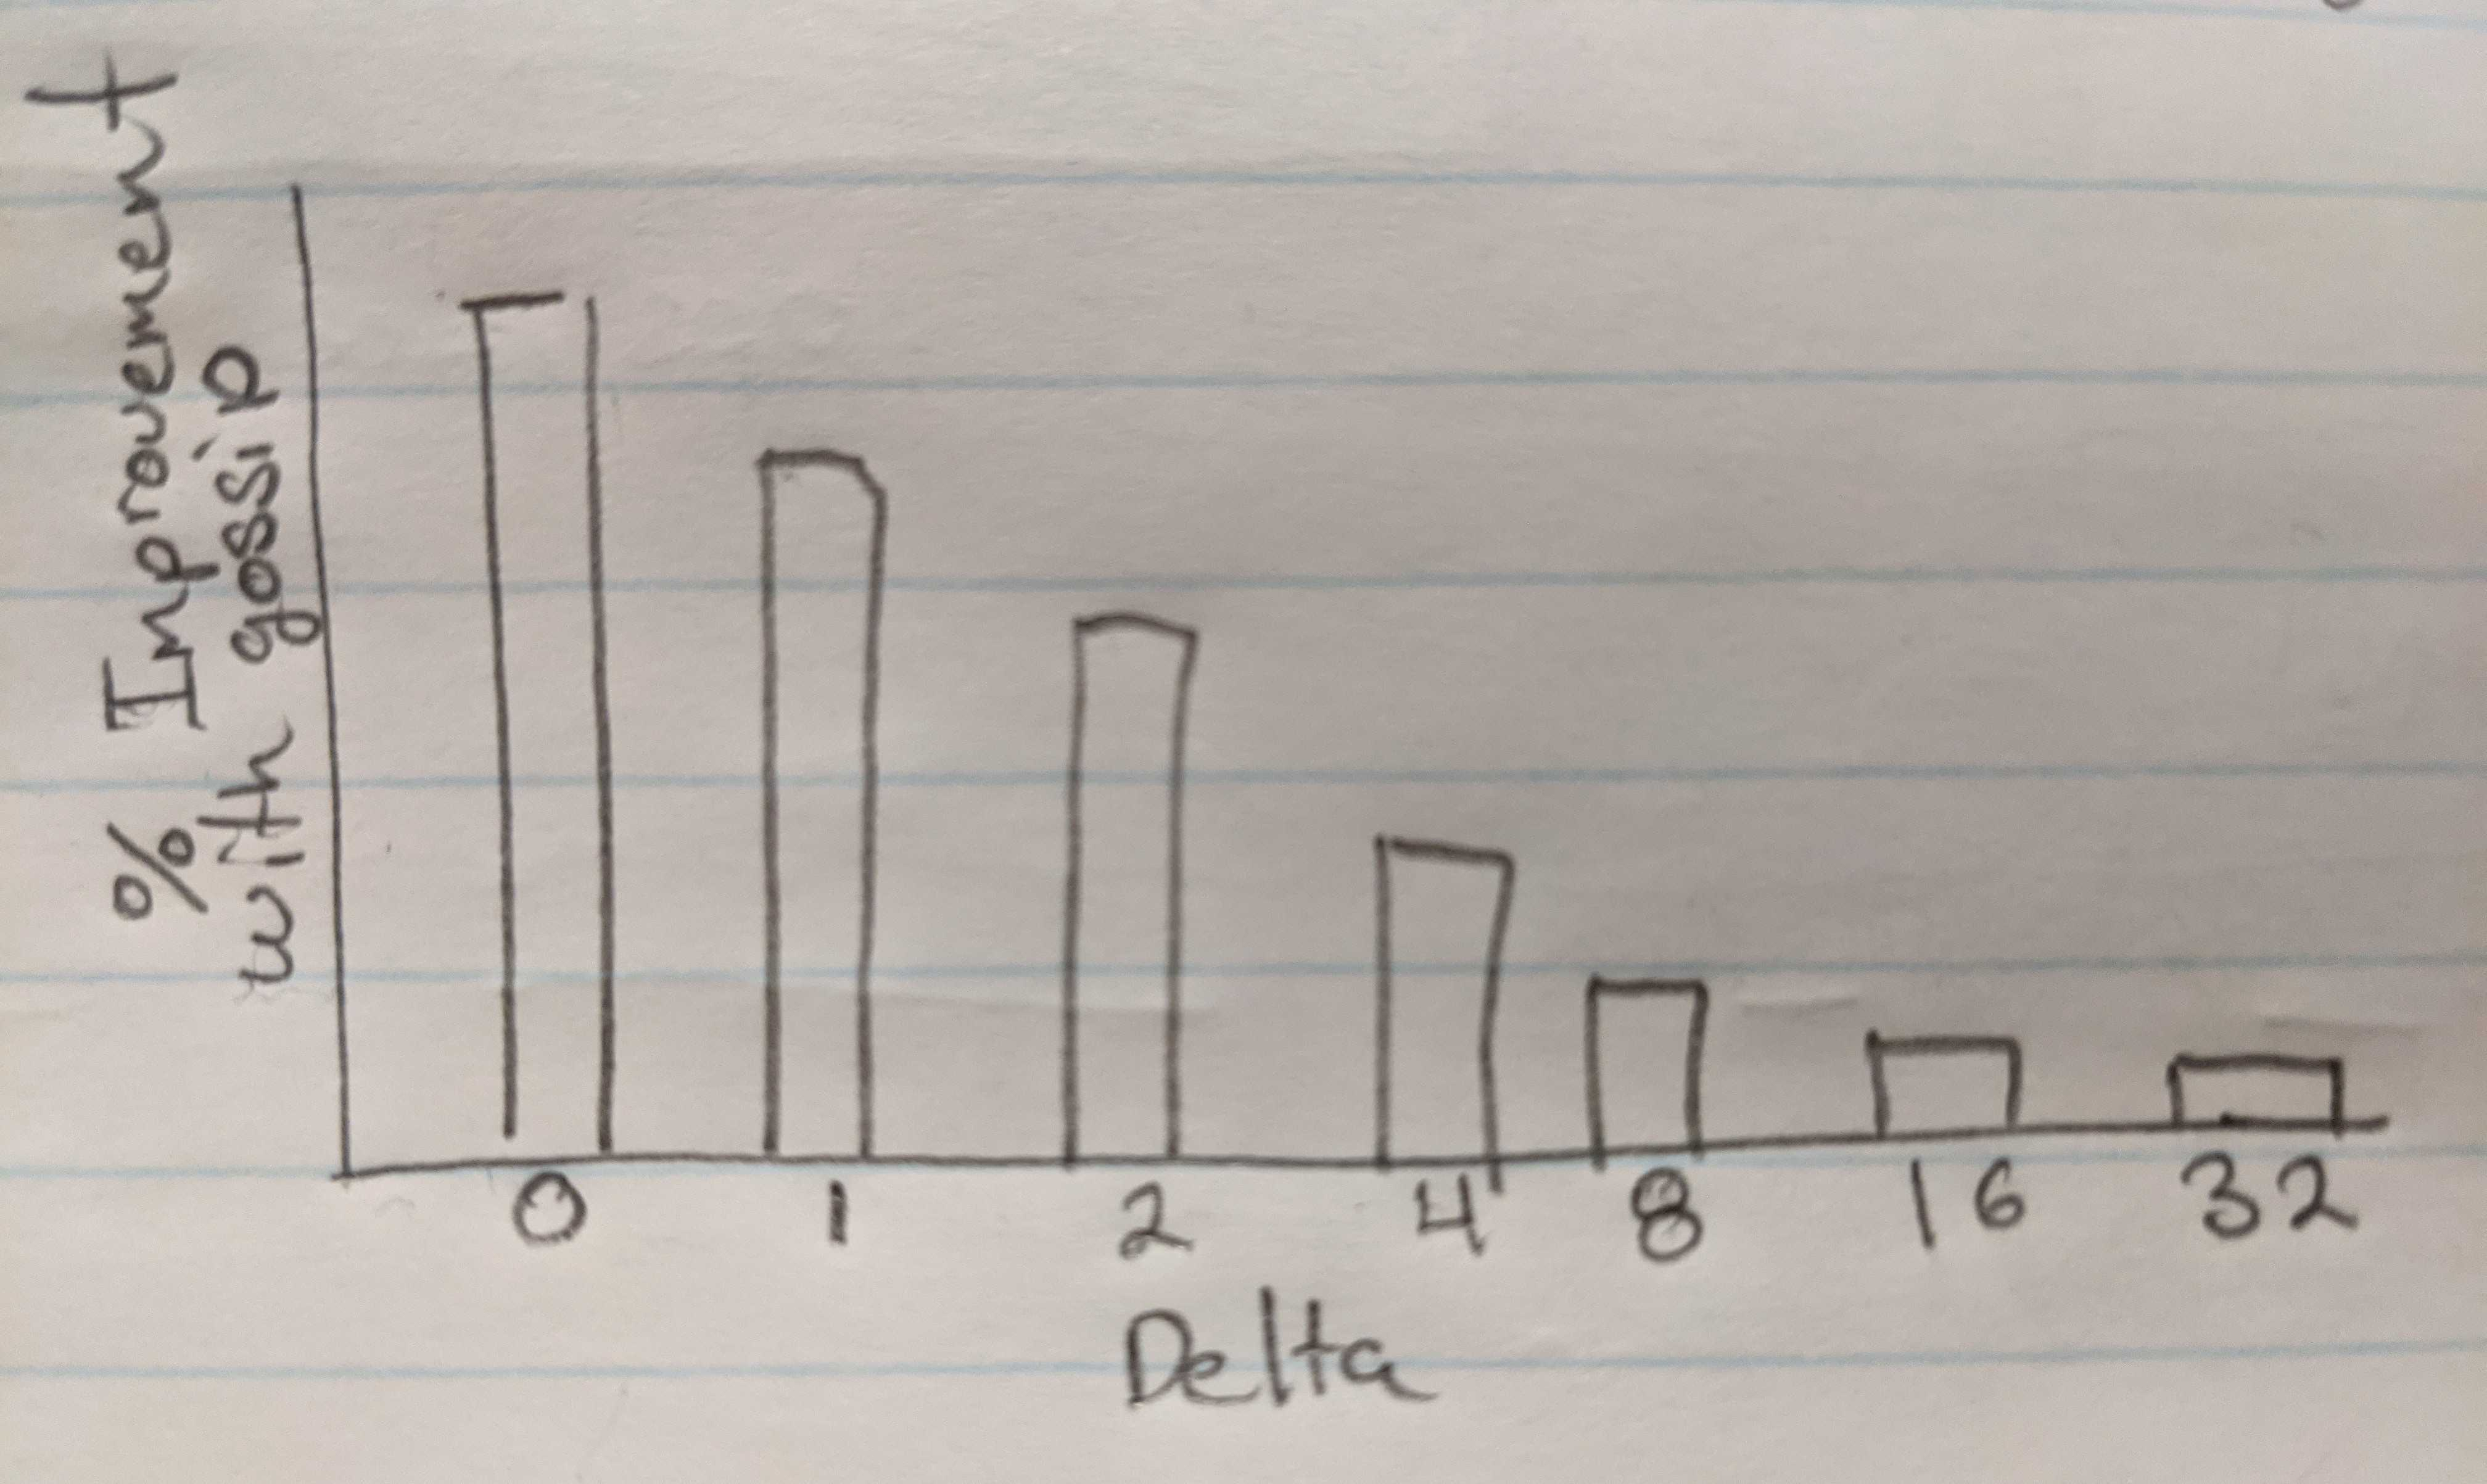
\includegraphics[width=0.45\textwidth]{fig/no_gossip.jpg}
%    \centering
%    \caption{\todo{Percentage improvement in load balancing decisions given
%%    50us load updates}}
%    \label{fig:no_gossip}
%\end{figure}

\subsection{Stale information}

Our experiments show that the frequency at which load is updated has a
significant effect on the quality of the decisions. However, there is a trade
off in terms of traffic overheads to keeping information up to date. As the
number of services increases, so too does the number of messages needed to
keep the information fresh. 

Given imperfect, or stale, information about remote servers, the
question becomes: \textit{when is redirecting requests a good course
  of action}? We submit that given reasonably predictable, but
potentially eccentric, request patterns, the correct course of action
is to act conservatively when conditions are manageable, and to react
quickly and decisively when request loads spike, i.e., in microburst
scenarios.  These constraints dictate a
compromise between inflating traffic and making sub-optimal decisions
with poor information.

\subsection{Information traffic reduction} 

Determining how often and when to send load information requires
careful consideration. If an update were to be propagated for every
request, that would be ideal from a decisions making perspective, but
the overall number of messages sent could inflate by the total
replication factor (2$\times$ or 3$\times$ in many cases).  Such
overheads are unacceptable for systems with requests in the thousands
or millions of requests per second as the cost of the information
quickly surmounts the goodput traffic. A key challenge in designing a
distributed in-network load balancer approach is to identify the most
critical information to send which ideally only produces a small
overhead in terms of state exchange messages.

%\subsection{Predictability}

Network operators generally want predictable behavior within their networks.
Given that distributed load balancing requires information to be spread, it
raises the risk of adding unpredictability to the network, specifically in
terms of overhead. An ideal load-balancing strategy would spread information
efficiently while allowing operators to set an overhead budget in terms of
bandwidth or messages which would correlate to a comparable increase in
performance. Predictability is highly important in heterogeneous systems where
multiple applications require guarantees about their apportioned network share.

\subsection{Heterogeneous rack configurations}

At datacenter scale the configuration for any application may vary wildly.
Individual service replicas may be co-located with resource-hungry applications.
Due to configuration differences applications might have varying processing
powers. Many applications are placed in VMs which execute on differently
powered hardware. Indeed, in the datacenter there is no guarantee that any set
of replicas is equally provisioned. Therefore any load-balancing strategy must
take into account this heterogeneity and apportion requests in response to the
real processing rate.

\section{Daronpon design}

The \systemname\ protocol resides within the ToR at each rack and is designed to
track server load by counting the number of outstanding requests for each
service running on that rack. Figure~\ref{fig:racks} illustrates the role that
ToRs play in our load balancing scheme.  When a request arrives at a ToR it
makes a load balancing decision. It either \textit{Admits} the request, or it
\textit{Redirects} it to another replica. The choice to either admit or
redirect is subject to the local load the service is currently experiencing
under the ToR (as understood by \systemname), and an estimation of the load
each replica has on remote ToRs. 

%If a request is admitted the ToR increments it's
%load counter for that service. Once the server complete the request
%and the response from that service passes back through the ToR the
%load counter is decremented. Each TOR has a perfect count of the
%number of outstanding requests underneath it (assuming reliable RPC)
%which it can use to request count of services running on remote racks
%are sent periodically which give ToRs approximate knowledge of their
%load.  Using this information ToRs make the decision to \textit{Admit}
%or \textit{Redirect} a request when it arrives. 

A ToR can only directly keep an up-to-date counter for the services running in
its rack. To make good load balancing decisions, fresh knowledge, and more
importantly knowledge of bursty behavior, is necessary.  Determining the
mechanisms for disseminating this load information is non-trivial.

We designed and tested a variety of different options for disseminating load
information in simulation and on an Amazon Web Services (AWS) testbed.  One
design gossiped load information periodically based on wall clock time, and
another gossiped on a per-request basis. Our results in simulation and on our
test setup demonstrate that both of these techniques require extremely high
overheads in terms of messages sent.  For example, our best results with
periodic message exchanges required updates polled every 25us. This resulted in
over a 2x overhead in terms of messages. Most of the information spread in this
case was redundant, and does not aid in mitigating bursts.  Further, it adds
congestion to the network, which reduces the maximum throughput, especially
during bursts, which is the opposite of our goal. An ideal load dissemination
protocol would quickly react to bursts while simultaneously generating little
overhead during burst events.

The \systemname\ protocol consists of two distinct but complementary messaging
algorithms.  The first is a logarithmic gossip protocol (described below) which
guarantees the reactive spread of load information when bursts occur, while
generating little overhead otherwise.  The second, an opportunistic
piggybacking protocol, spreads load information between ToRs when requests are
redirected. We find in our evaluation that our log gossip approach prevents
large queue build ups, while our piggyback approach greatly reduces latency in
the common case.  These results are outlined in detail later in this paper.

\begin{figure}[ht]
  \centering
    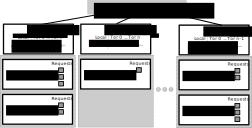
\includegraphics[width=0.8\textwidth]{./figure/daronpon/racks.pdf}
    \caption{High-level overview of \toolname. Each ToR tracks
    outstanding request for services running in its rack, and
    maintains approximate counters for remote ToRs hosting shared
    replicated services.} 

  \label{fig:racks}
\end{figure}

%\subsection{Gossip Periods}
%\begin{figure}[ht]
%  \centering
%    \includegraphics[width=0.45\textwidth]{fig/diffgossip.pdf}
%    \centering
%    \caption{Different gossip periods from 1\/2 RTT to 16 RTTs. Using constant service time 25 us} 
%  \label{fig:diffgossip}
%\end{figure}

%Information about remote load counters is the key factor in making
%redirection decisions. Out-of-date load information is of low utility
%over time as its accuracy decreases. Therefore, the
%load gossip period has a remarkable effect on the overall performance.

%We tested the effect by running different gossip periods.
%After each run the period of gossip messages is doubled, starting at 25 us. 
%Figure~\ref{fig:diffgossip} shows the resulting
%trend when our servers are stressed at 30k request per second. 
%While doubling the gossip period, we can see 
%a linear performance degradation on 95th, 99th, and 99.9th percentiles latency
%starting at 100us, i.e. 1 RTT.
%The 50th, 95th, 99th, and 99.9th percentiles latency increase
%4.4\%, 26.9\%, 42.7\%, 58.3\% with 32x gossip periods. 

%%
%A marginal benefit is found at any gossip periods as a local redirections
%require a queue depths of 1 or greater, and even with poor information
%the probability of a redirected request landing at a less stressed
%server is sufficient enough for a performance benefit. 



% \sg{The aggregate number of gossip messages grows exponentially with the number
% of services running under each TOR. We should consider pointing out
% some mechanisms which might amortize the cost of these messages.}

% \begin{figure}[t]
%   \centering
%     \includegraphics[width=0.45\textwidth]{fig/load_spread.pdf}
%     \centering
%     \caption{ Request latency response to gossip message frequency
%     with servers loaded at 70\%. Exponential increases in frequency
%     lead to linear increase in performance. ~\todo{make off values
%     line up with ~\ref{fig:delta}} ~\todo{average over more runs, this
%     is taken over 10}.
% }
%     \label{fig:load_spread}
% \end{figure}

%\subsection{Load Delta}
%\begin{figure}[ht]
%  \centering
%    \includegraphics[width=0.45\textwidth]{fig/diffdelta.pdf}
%    \centering
%    \caption{Different load delta values to avoid aggressive redirection. Using constant service time 25 us} 
%  \label{fig:diffdelta}
%\end{figure}

%Figure~\ref{fig:diffdelta} shows microbenchmark results 
%of requests latency varies across delta values. 
%Applying ToR redirection with small delta values improves performance. 
%However, larger delta values avoid aggressive redirections but they hurt
%the performance by missing redirection with potential benefits.
%We can see the tail latency substantially increased after delta value of 10 under 
%a 35 KRPS request rate.
%The 50th, 95th, 99th, and 99.9th percentiles latency increase 
%23.0\%, 20.9\%, 13.3\%, and 12.5\% when delta value increase from 10 to 80.

%\begin{figure}[ht]
%  \centering
%    \includegraphics[width=0.45\textwidth]{fig/diffdelta0to10.pdf}
%    \centering
%    \caption{Zoom-in view of delta values from 0 to 10. Using constant service time 25 us} 
%  \label{fig:diffdelta0to10}
%\end{figure}

%As shown in Figure~\ref{fig:diffdelta0to10} increasing delta values
%from 0 to 10, we saw a smaller but observable increase on latency.  We
%observed 22.0\%, 19.9\%, 14.2\% increase on the 50th, 95th, and 99th
%percentiles latency.  The increase on 95th, and 99th percentiles
%latency starts at delta value = 5.

%We saw a local minimum of request latency at delta value 2 and 3 at medium request rate 30kRPS.
%Using delta=2 gives us 7.1\%, 8.2\%, 7.8\%, and 7.1\% improvements on
%on 50th, 95th, 99th percentiles, and 99.9th percentiles. Throughout
%our experiments we use a delta value of two as our local optimum.


%\todo{Load delta can be used as a way to reduce the total number of
%packet redirections. Should we choose to add redirections to the cost
%of our algorithm we want to show how using a load delta can decrease
%that}

\subsection{Microbursts}

Figure~\ref{fig:microburst} (top) shows an example of a microburst. In this
case, requests are issued at a Poisson arrival rate by multiple clients.  The
peaks show outstanding requests from the perspective of a ToR instrumented to
track request counts. In this case, when requests queue, that queue grows
without bound, even though other replicated services are available to process
this influx of requests. This has a dramatic impact on the tail latency of the
requests in the burst, and also the overall mean request time. A typical
request incurs longer wait times due to decreased overall system throughput.

In Figure~\ref{fig:microburst} (bottom) the queue builds up with our
logarithmic gossip mechanism enabled. Each \textit{red X's} on the chart
represents a point at which the load on the server is gossiped.  Note that when
peaks occur, and a gossip is sent, the load is quickly spread to other servers.
This increases overall system throughput and decreases tail latency. This
strategy, however, is not perfect. At low load the benefit of redirecting
requests is minimal. For example, when the number of outstanding requests is
just one or two above a remote service, and so redirection reduces overall
performance.

The age of the gossiped information complicates the act of redirecting. The
remote information on remote hosts is at least a few microseconds out of date.
Given the few microsecond budget our requests have to begin with, the benefit
of redirection quickly evaporates if even a few request arrive from the point
in time at which the load information is sent.  This leads to unnecessary
redirections and high overheads in terms of gossip messages which do not
ultimately deliver useful information. This overhead can be mitigated by adding
a threshold which prevents gossip messages from being sent until the number of
outstanding requests has exceeded a given threshold.  Our proposed log gossip
technique for curtailing this overhead is described in the following section.

%Gossip messages consume and packet processing time.  Therefore their
%frequency must be chosen with care as to not introduce significant
%variance into the system. The majority of data center packet drops
%occur on south facing ToR egress to the host.~\cite{jupiter-rising},
%our approach only increases bandwidth above the ToRs which allows for
%a higher gossip bandwidth budget prior to it causing significant
%interference. Gossip messages are small, (approximately
%64 bytes depending on the number of services), which reduces aggregate
%bandwidth consumption.

%Our testbed results use gossip messages as
%frequently as 10us without any noticeable interference on 40Gbps
%networks. As network speeds increase we anticipate that the available
%bandwidth for background traffic which improves the performance of
%running services will increase.


\begin{figure}[t]
  \centering
    \includegraphics[width=0.80\textwidth]{./figure/daronpon/burst.pdf}
    \centering

    \caption{Microburst with no mitigation (top) vs. with
    logarithmic gossip load balancing enabled (bottom)}

  \label{fig:microburst}
\end{figure}

\subsection{Packet flow}

The \systemname\ load balancers are stateful and act per request.
Figure~\ref{fig:load_balancer} provides a high level message flow diagram of
this system.  When requests arrive, \systemname\ executes the admission
protocol. Requests are admitted only if the local service has the minimum
observable global load. A load tracker keeps counters for each global service.
Local counters are up-to-date, while remote counters are learned via gossip and
piggyback messages.  When a request is admitted, the ToR increments its load
counter corresponding to that service.  When a response passes back through the
ToR, that service has its local counter decremented.  If, when a request
arrives, the local load of a service is not the global minimum, the request is
redirected. The redirected request is then sent to the service with the lowest
load, based on the ToRs' local load tracker (see
Section~\ref{subsec:piggyback}).  Redirected requests have load information
attached to them. The attached load consists of request counters for the
intersection of services the ToRs share.  Therefore, the overhead per
redirected request is variable as per the systems' configuration.

Increments and decrements in local load are tracked by a gossip monitor (see
Section~\ref{subsec:gossip}). The job of the gossip monitor is two-fold. First,
it identifies bursts. When load spikes the monitor broadcasts gossip messages
to let other ToRs know it is experiencing high load. Second, it identifies
valleys. Load balancing schemes which use potentially stale information are
known to exhibit herding behavior, a condition which leads to sub-optimal
queuing behavior~\cite{dahlin_stale_info,mitzenmacher_old_info}. When load
drops sharply, gossip messages are also generated to announce that a service
has spare processing capacity.

\begin{figure}[t]
  \centering
    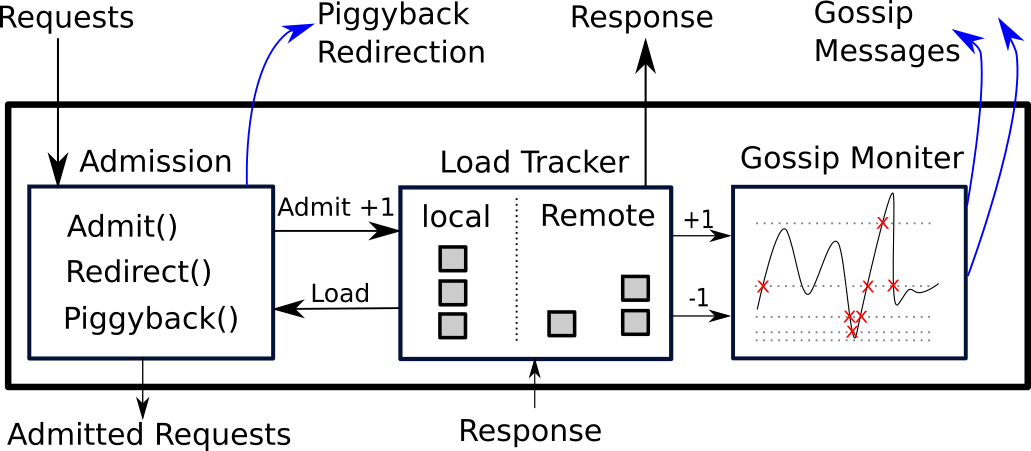
\includegraphics[width=0.80\textwidth]{./figure/daronpon/load_balancer.pdf}
    \centering

    \caption{ %% 
        %%
        Key functionality and message flow of \toolname.
        Incoming requests are either admitted or redirected.
        Redirected requests spread load information via piggyback.
        Load is updated upon admission, and response.  Gossip messages
        are issues when load breaks a logarithmic threshold.}

  \label{fig:load_balancer}
\end{figure}

\subsection{Logarithmic Gossip}
\label{subsec:gossip}

\begin{figure}[t]
  \centering
    \includegraphics[width=0.90\textwidth]{./figure/daronpon/log_thresh.pdf}
    \centering
    \caption{The percentage of gossip messages generated by a
    logarithmic gossip mechanism as a percentage of overall traffic.
    Collected from runs of 96 KRPS.} 
  \label{fig:log_thresh}
\end{figure}

The \systemname\ algorithm for generating gossip messages has the primary goals
of reacting quickly to bursts while consuming little overhead in terms of
additional messages.  In an earlier design, ToRs gossiped load information every
25 $\mu$s. This approach has the advantage of providing highly updated load
information, but it incurred scalability bottlenecks as the number of ToR
increased, since the 25 $\mu$s gossip contends with request goodput for link
bandwidth.

To compress the number of messages, we adjusted the gossip protocol to only
send messages on exponential changes in load. We use powers of two as our
exponential interval, and we choose two both for its effectiveness in practice
and for its ease of computation, only requiring bit shift operations. To our
knowledge, no commodity programmable switch can compute floating point
arithmetic in the data path~\cite{challenging_programable}.

Each exponential step increases the bounds in which server load can fluctuate
prior to a gossip message being issued. For instance, if the load were to
increase from 1 to 2, a gossip message would be broadcast to all other servers
with the replicated service that crossed this threshold. In this message, load
information for all other shared services is added. When the boundary of two is
crossed, and the value of two is sent, this ToR will not issue another gossip
message until the load on the service rises by a power of two to four, or falls
back down by a power of two to one.

%%
%% Sorting microbursts by size
%%
The above described protocol has several benefits. First, it sorts microbursts
by magnitude without adding significant packet overhead. Given that small
fluctuations may occur at rapid pace, it is important to give priority to
bursts with larger magnitudes. Other methods of achieving this goal such as
piggybacking can lead to stale information, which has significant differences
to ground-truth values, even when a server is experiencing very
high load.


%%
%% Reduces congestion when bandwidth is needed
%%
The protocol also decreases the number of gossip messages sent during 
bursts, which reduces the overall strain on the system when resources
are at their tightest. This is an issue with gossip strategies that
operate periodically (e.g. at preordained wall clock times)
or are issued at some constant ratio
to requests (e.g gossip every 5 requests).  When request rates
are low, gossip messages are automatically sent with a higher frequency
per number of requests which allows for better decision-making at lower
request rates.
%%
%%Aggregation of requets
%%
ToRs have the advantage of being an aggregator for the load of an
entire rack. Were we to implement our solution on end hosts, each host
would need to gossip its load to every other host. Using ToRs, the load of
each server in a rack is known explicitly and is gossiped in its
entirety, assuming the rack sees both requests and the associated
responses.

%%
%% Fast reaction
%%
Other approaches which use load information collected from end hosts
themselves suffer from additional delays in responding to load spikes,
as the knowledge of load must be transmitted to the balancer before it
can react. Our approach reacts to load as soon as a request is
admitted. This allows for precise load balancing decisions to be made
at sub-RTT time scales. 
%%
For instance, in a Fat-Tree with two ToRs connected by a single
aggregate switch, the distance traveled by load updates is halved in
comparisons to a host based solutions (e.g. Tor-Agg-Tor vs
Host-Tor-Agg-Tor-Host). This approach is not limited to Fat-trees,
as
many networks use ToRs, however our ToR-based approach always results
in two hops less than an host based approach.

%% %Approximate measure of load, but fast react %
We give up precise, up-to-date measures of load on the host, something we can
only get with precise application level knowledge and host control, and instead
use counters to estimate server load in the ToR. This imposes lower tracking
overhead, and performs nearly as well as highly tuned approaches which report
server load directly~\cite[Figure. 15 (proactive)]{racksched}.

%%
%% Threshold
%%
This algorithm decreases the number of gossip messages
significantly, and can be greatly improved by carefully considering a
lower bound at which to disable the mechanism entirely.
For example, setting a lower
threshold such as $t$ implies that below an outstanding request count of
$t$ a ToR will not gossip information.


Figure~\ref{fig:log_thresh} shows the percentage of messages gossiped relative
to the requests processed for different threshold values.  Note that the
default values of 0 and 1 have an overhead of around 30\% of the request rate.
Redirections of requests at these levels of outstanding request sees little
benefit in terms of performance as at any reasonably high request rate, the
depth of remote queues have changed since the remote data was received making
the choice stale. By increasing the threshold to four, the overhead in gossip
messages is reduced by a factor of ten down to around 2\% when our system is
around 70\% saturation. See Section~\ref{sec:service_time} for a comprehensive
evaluation of gossip overhead. Increasing the gossip threshold beyond four
significantly reduces overhead down to around 0.02\%, however this comes at the
cost of only identifying bursts of size eight and greater which significantly
effects our reductions in 99th percentile tail latencies.

%%
%% Staleness
%%
One limitation of our algorithm is that it provides no liveness
guarantees with regard to the freshness of the load information
announced. For instance, a server which maintains an outstanding number
of requests between 4 and 16 for $n$ requests will not issue a gossip
until either threshold is crossed. While this is unlikely in practice
due to the small range and short duration of requests, there is no
guarantee. This can become an issue for extended periods of load when
the number of outstanding requests is deep (e.g. 128 to 512).

\subsection{Piggyback}

\label{subsec:piggyback}
\begin{figure}[t]
  \centering
    \includegraphics[width=0.90\textwidth]{./figure/daronpon/breakdown.pdf}
    \centering
    \caption{Performance breakdown of gossip and piggyback mechanisms.
    Lower values are better.} 
  \label{fig:breakdown}
\end{figure}

Using logarithmic intervals for gossip messages, we can clearly identify and
mitigate bursts.  While this is advantageous in general, there is still
additional performance to be gained.  With gossip enabled, the percentage of
redirected requests is around 22\%. Each one of these redirected requests is
sent from the redirecting ToR to the receiving one, and therefore has the
ability to report the load information on the ToR that performed the
redirection.  We refer to this method of attaching load information to
redirected requests as piggyback, and using redirection to spread information
provides significant advantages in the common case.

In contrast to the centralized approaches in both Racksched and
R2P2~\cite{racksched, r2p2} piggybacking information load on requests
is not a sufficient mechanisms for learning about remote load. This is
because our load balancer is decentralized, which means that our load
balancers do not see load information updates from every request.
Unlike our logarithmic gossip mechanisms, it provides no guarantees
about its operational bounds. Using gossip messages exclusively
provides no guarantees that any specific server will have information
propagated to it as only the server which is redirected to receive
fresh information.

In the case of these centralized solutions, each request returns some
information to the scheduler. In the distributed case, there is no liveness
guarantee with regard to redirections, and indeed, information can become
arbitrarily stale. We therefore consider our piggyback algorithm to
opportunistic, only aiding in the common case when load is low, but when making
precise redirections will still improve throughput and provide
lower latency.

Piggybacking load has the advantage that it is responsive proportional to the
request rate of the system. As the number of requests per second increases so
to does the rate at which information is spread between ToRs. Further, it has
the advantage of introducing a small amount of overhead. Rather than incurring
the cost of an entire load information update, this only adds a few bytes to a
custom header injected at the ToR.

Figure~\ref{fig:breakdown} shows a performance breakdown of the two parts of
our protocol. At low request rates the gossip protocol does not provide much of
a performance benefit in relation to the piggyback method. However as the
request rate, and variability, of the system rises (e.g. to 102 and 105
thousand requests per second), the gossip mechanism provides the majority of
the gains as it detects the peaks which increase tail latencies the most.

\section{Implementation}

We have deployed \systemname\ in the AWS cloud environment, with service
instances hosted in VMs connected via Elastic Network Adapter (ENA) virtual
NICs. These instances use the Data Plane Development Kit (DPDK).

\paragraph{Components:} Our deployment consists of three components: DPDK ToRs,
DPDK clients, and servers with default Linux networking stacks relying on UDP
for application messaging. DPDK is a kernel bypass networking library which
allows for high throughput and low latency packet processing in user
space~\cite{dpdk}. DPDK ToRs emulate ToR switches with limited latency overhead
($<$ 1 microsecond).  Ideally, we would implement our algorithm on P4 switches,
however to our knowledge no cloud providers allow for customers to offload
custom programs to programmable switches at this time.  We implement our
clients using DPDK for lower latency and precisely controllable request rates.
These traits are important as AWS's ENA NICs do not have hardware timestamping
available to users.  Our DPDK clients can generate hundreds of thousands of
requests per second with a single virtual core. These UDP-based servers
represent services relying on the standard Linux networking stack. We choose to
use UDP as the transport because it allows us to redirect request atomically
without connecting multiple packets together and redirecting as a group, though
this could be supported as future work.

\paragraph{\toolname\ DPDK ToRs:} Our DPDK ToRs use an arbetry number
of cores to forward requests/responses and a single core to gossip
load information. Redirecting involves header manipulation, tracking
load information using hashtable table lookups, and counter
increment/decrement operations. The operations we used in these DPDK
ToRs are carefully chosen to be simple, and within the capabilities of
programable switches to compute.

\paragraph{Custom packet headers:} We our inject custom header after
the IPv4 UDP header. It consists of a unique request ID for each
request, which is used to track lost packets and measure end-to-end
latency. A service type field differentiates services, e.g Memcached
and RocksDB.  Additionally, the IP and ports describe addresses of
replicas which implement other copies of the service.  We assume that
clients know the server replica addresses by asking the cluster-level
replication manager, e.g., Google's Slicer or Facebook's Shard
manager~\cite{facebook_shard,google_slicer,microsoft_service_fabric}.
Gossip messages are also based on UDP, and load information is
appended after the UDP header.  The header contains a list of server
addresses, load counters, and its corresponding service types for all
servers under a ToR switch. 

\section{Evaluation}
\label{sec:eval}

%define setup variables here
\newcommand{\instances}{9 }
\newcommand{\racks}{3 }
\newcommand{\servers}{3 }
\newcommand{\servercores}{1 }
\newcommand{\tors}{3 }
\newcommand{\torscores}{8 }
\newcommand{\clients}{3 }
\newcommand{\clientcores}{1 }

We evaluate \systemname in on the Amazon Web Services cloud (AWS
\texttt{us-west-2} region). In this section, we describe these experiments and
the resulting conclusions.

\subsection{Experimental setup}

%\textbf{Testbed:} %
We use \servers \texttt{c5n} instances as servers, \clients as clients, and
\tors as software ToRs. All instances are placed in a single cluster placement
group for predictable low latency. The mean RTT latency between every instance
is about 50 microseconds.  In this setup, we configure three server machines,
three clients, and three DPDK software ToRs. This simple configuration emulates
a datacenter network in which each ToR has exactly one service running
underneath it.  Services are deployed to servers using the stock Linux
networking stack.  While this does incur higher latencies as compared to
DPDK-based kernel bypass stack, we note that it is representative of many
datacenter applications.

%why did we chose to do it on AWS?-> it's a real cloud  why did we
%chose to use DPDK software ToRs-> because we don't have access to the
%ToR to make latency more tractable we use cluster placement group

We implement the \textit{random} service selection as a simple and standard
baseline. Client-based ``power of two'' approaches are not comparable because
they require excessive probing of server load, incurring at least one RTT per
probe. This load creates unnecessary congestion on the DPDK ToR instances and
ENA virtual NICs.  \toolname\ can be easily extended to implement the ``power
of two'' approaches on ToRs and the performance should be similar, based on
simulation results reported in LSQ~\cite{lsq}.  Each client randomly selects a
service designation. In the random configuration, requests traverse our DPDK
software ToRs with our load balancing mechanism off, and they flow through to
their selected destinations. We compare \toolname\ random in
the following experiments.

\subsection{Workloads}

We evaluate our load balancing approach with a simple request-response
application, in which the time spent on the server is computed based on a
statistical process.  In our evaluation, we generate requests according to two
statistical distributions, one of which generates application-level requests
and is run on DPDK-based clients, and another which generates emulated service
times. Clients generate requests based on open-loop Poisson arrival using the
standard random library.  Servers distributions are split into different
distribution categories, each of which has its own separate parameters. These
include constant time, bimodal, and exponential distributions. 

Each server is loaded with an equal number of requests (in expectation)
drawn from common request rate distributions, as described next.
Our goal in using these distributions is to demonstrate that
our technique of using outstanding requests (blind to the underlying
service distribution) works in general, without the need to tune
our load balancer for each application.  Both our gossip protocol and
piggyback protocol are enabled in each experiment. The lower threshold
on our gossip protocol is 4.

\noindent\textbf{Constant:} In this distribution, all requests take 25 $\mu$s to
complete on the server.  In the server, a work thread busy-polls the time until
the 25 $\mu$s deadline has passed to emulate application-level service times.
This workload is indicative of many highly tuned key-value stores with strict
SLOs~\cite{memcached,rocksdb}.  Our servers experience additional latency
overheads from the Linux networking stack.  Our choice of this constant latency
is intended to be representative of a performance-tuned microservice which
performs a fixed amount of work per request.  To provide a sensitivity analysis
to this choice of constant, Section~\ref{sec:service} provides an overview of
our system performance across constant service times separated by an order of
magnitude above and below 25us.

\noindent\textbf{Exponential:} To generate an exponential distribution we use the
standard C++ random library. We set the mean to 25 $\mu$s with a standard
distribution of 40,000. These parameters generate tails of up to 400 $\mu$s
which is indicative of many applications that may be subject to blocking, such
as occasional writes to disk or the invocation of a blocking RPC to another
machine.

\noindent\textbf{Bimodal:} Our bimodal service times are distributed into two
categories. 90\% of the requests take 13 $\mu$s and 10\% are 130 $\mu$s.  We
choose this distribution as the mean value is close to 25 $\mu$s. This
distribution is aimed at emulating longer and less frequent tasks such as
writes and scans in certain key-value store workloads or even garbage
collection events in the runtime.

\subsection{End-to-end experiments}

\begin{figure*}
  \includegraphics[width=\textwidth,height=4cm]{./figure/daronpon/homo.pdf}
  \caption{99th percentile latency improvements on three common
    service distributions (Constant, Bimodal, Exponential). Each
    server is provisioned with homogeneous processing power.}
  \label{fig:homo}
\end{figure*}

We test the effectiveness of our load balancing technique by running it against
random replica selection alternatives on the aforementioned workloads.
Figure~\ref{fig:homo} shows the relative performance gains across these
workloads at the 99th percentile latency. In this configuration, each of the
servers has identical processing capacity for each service.  We consider this
idealized and homogeneous configuration because of its simplicity.

\systemname sees the most relative gain over random when skew in the workloads
is common. At high loads, request variation occurs at higher degrees for
multiple reasons. First, the Poisson arrival process on our clients has a
higher probability of generating bursty sequences of events at higher load.
Second, hypervisor and NIC hardware on AWS contributes to the bursty arrival of
requests because of the underlying batching behavior.  These forms of
burstiness is largely out of our control as we do not have direct access to
AWS's hardware configuration.  Finally, as rates increase, more batching
happens in the Linux kernel networking stack. This leads to sharp decreases in
the number of outstanding requests. 

\toolname\ sees the largest benefits in the bimodal and exponential
distributions and the long service times cause significant and frequent queuing
on the end hosts. The logarithmic gossip protocol reacts quickly to these
changes under load and steers requests away from the servers which are running
long average request times.  In our homogeneous experiments, the average value
for number of outstanding requests is four in our constant distribution, with
frequent peaks of up to 80 outstanding requests when \toolname\ is disabled.

\noindent\textbf{Constant:} Figure~\ref{fig:homo}A shows our approach provide benefit
on tail latency starting at 78 Krps (kilo-requests per second).  This constant
workload gives \toolname\ the fewest opportunities to load balance effectively
as the random distribution of requests, each with a static service time, should
be approximately even. In this distribution, the benefit is found in the load
fluctuations. At high request rates, other mechanisms such as Linux's request
batching, have more of an effect on queuing.

At the highest request rate that a single vCPU core can handle, the latency
improvement of \systemname at the mean is 1.32x and on 99.9th percentile is
1.62x.

\noindent\textbf{Bimodal:} In Figure~\ref{fig:homo}B, we see the disparity between
random service selection and \toolname. The service time dispersion provided by
bimodal distribution causes noticeable request queuing when a long service time
request occupying a service.  Logarithmic gossip messages are ideal in this
case as they quickly react to the skew in load.  Further, in this distribution
the probability of finding an under-utilized replica is relativity high.  

\noindent\textbf{Exponential:} Figure~\ref{fig:homo}C shows the throughput and
latency gains on an exponential server distribution. Our benefits are most
noticeable here as the exponential distribution leads to the fastest disparity
in load. In this case, a single request on the exponential distribution can
lead to significant queuing on a given server. Our latency improvements at 102
Krps is 1.61x in the mean and 1.54x at 99th percentile.

\subsection{Heterogeneous server configurations}

\begin{figure*}
  \includegraphics[width=0.9\textwidth,height=4cm]{./figure/daronpon/hetero.pdf}

  \caption{Throughput and latency improvements with skewed processing
    capacity in a heterogeneous server configuration. \toolname\
    scales linearly with with the aggregate processing capacity
    available.}

  \label{fig:hetero}
\end{figure*}

The placement of replicated services is subject to the cluster
scheduler~\cite{facebook_shard,google_slicer,microsoft_service_fabric}.  The
placement of individual services may be tightly coupled to a single rack, or
distributed to multiple racks.  Additionally not all replicated services may be
configured using identically powered instances. Some may be provisioned with
different core counts, memory, and potentially different OS versions.  Finally,
should rack-level scheduling be utilized such as Racksched or R2P2, the
individual rack level throughput may differ below the operating domain of
\toolname.

To show the generality of our approach in situations where replicated
applications differ in their throughput capabilities, we configure one out of
our three servers to run using twice the processing capacity (i.e., two CPU
cores rather than one). In this setup, clients otherwise operate identically to
the homogeneous configuration.

Figure~\ref{fig:hetero} shows the performance gains from enabling \toolname\ on
our heterogeneous testbed. In this test, the server with twice the processing
power of the other processes requests twice as quickly.  Our random client
takes no measure of queue depth, and therefore does not adjust to this excess
compute power. Its performance is only marginally better in this case, as the
request which its probabilistically sends to the doubly provisioned server are
processed more quickly. 

\toolname\ apportions load to servers in precise relation to their processing
power. Our results from this test show that \toolname\ exhibits ideal scaling
in this small test. Where three vCPUs can process about 100Krps, four can
process about 133 Krps with the same 99th percentile tail latency. When running
in a heterogeneous configuration, the proportion of gossip and piggyback
request remains approximately the same as in the homogeneous case. The gossip
mechanism is triggered periodically as the request on the faster servers drains
below its current threshold, however this periodic variance occurs on the same
order as the natural fluctuations in load. Redirections also occur at
approximately the same rate, however they are almost entirely directed at the
over provisioned server.

Ideally, we would demonstrate the scalability of \toolname\ across many racks
with more services. We see this heterogeneous result as a proof of concept that
our approach can scale approximately linearly with available processing power.
We expect this result to hold as our approach is similar in style to
theoretical approaches for distributed load balancing which are proven to
provide linear scaling while using incomplete local information to balance
load~\cite{lsq}.

\subsection{Service time sensitivity analysis}
\label{sec:service_time}

\label{sec:service}
\begin{figure*}
  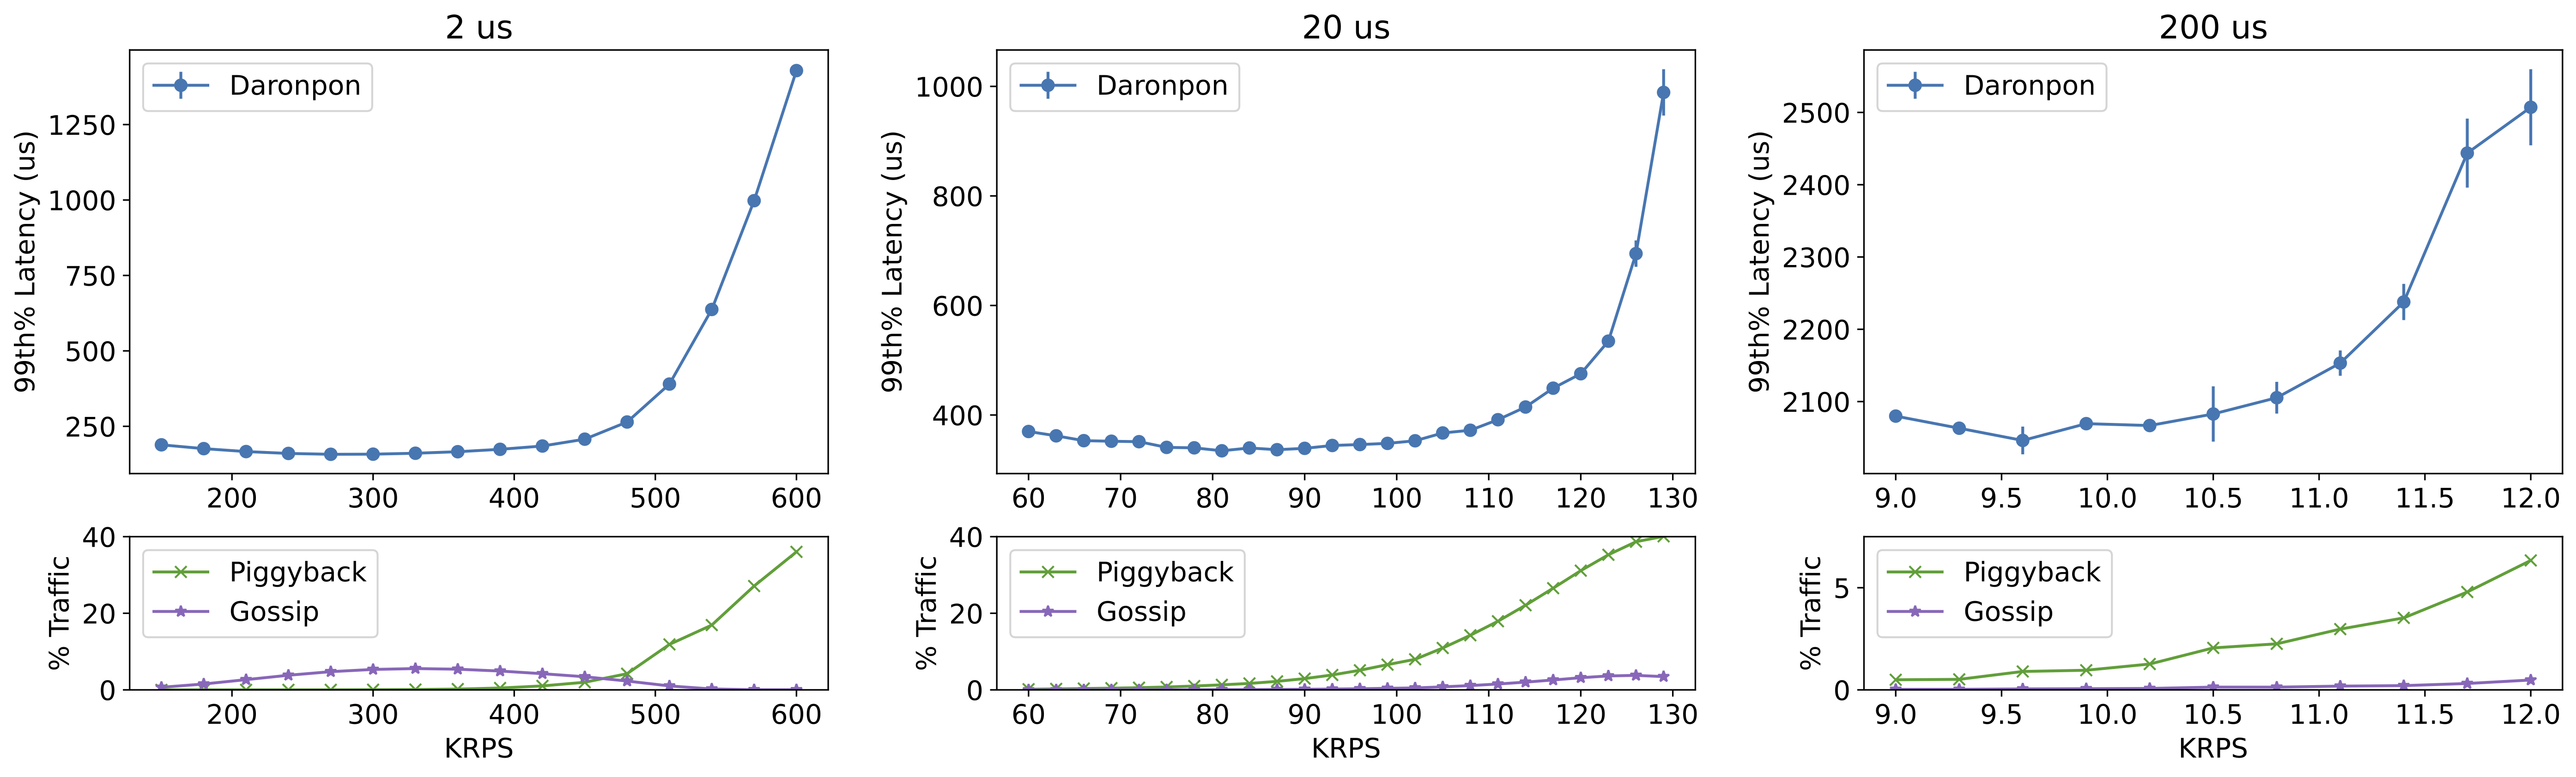
\includegraphics[width=\textwidth,height=4cm]{./figure/daronpon/service.pdf}

    \caption{Service times across three orders of magnitude (2us, 20us,
    200us). \toolname\ provides relative improvements with similar
    overheads in terms of piggyback and gossip messages at each
    service time. 
    \TODO{This needs to be changed to EWMA results along with the text.}
    }

  \label{fig:service}
\end{figure*}

We choose 25 $\mu$s as a baseline service time for an example microservice,
however our load balancing techniques are not limited to timescales centered
around this constant. To demonstrate that \toolname\ can provide throughput and
latency improvements across differing service times, we vary a constant service
time by three orders of magnitude across three experiments: 2 $\mu$s, 20
$\mu$s, and 200 $\mu$s.  Lower mean service times mean that our Linux servers
are able to process more requests per second, and vice versa.  It also means
that the number of outstanding requests from the view of our software switches
is higher on average.  We show the effect this has on the logarithmic gossip
mechanism, and the proportion of messages which are redirected at each request
rate.

Figure~\ref{fig:service} shows the performance gains \toolname\ achieves in
each case. At 25 $\mu$s (see Figure~\ref{fig:service}, middle), our mechanisms
operate as shown in prior experiments with the maximum gossip overhead reaching
no more than 3\% at peak system load. The number of piggyback messages grows
with the request rate. This is because at higher rates more bursts occur, and
thus the opportunities to load balance increase.

Near peak load, the number of redirections reaches approximately 40\%, and
while this results in the highest performance, it does incur an additional tax
on link bandwidth. We devised a threshold similar to the baseline used in our
log gossip mechanism which required the value of a remote queue to be lower
than that of the local queue by a specified delta before a redirection occurs.
In each of our experiments, this delta value is set to 0, which means that the
minimum replica is always selected. Choosing delta values above 0 resulted in
significantly lower numbers of redirections, with a value of 8 resulting in
piggyback messages being generated around 6\% of the requests, but also
resulting in only a 4\% performance gain over the random policy. In this way,
redirection mitigation is a strict trade-off of performance, resulting in lower
tail latencies at the cost of additional bandwidth.

At 2 $\mu$s, \toolname\ provides less relative improvements than at 25 $\mu$s.
This is due to the increased average queue depth, and the effect it has on our
log gossip mechanism.  Statically, using powers of two as a means to compress
the number of messages is worse in this case than when the outstanding requests
are lower. This is because at lower thresholds powers of two are exceeded more
frequently. At ranges of 64 and above, bursts need to be quite significant
before they result in a gossip exchange.  As seen in the lower part of
Figure~\ref{fig:service}, 2 $\mu$s gossips as a percentage of the overall
traffic starts to fall around 300 Krps.

Here we consider that an additional mechanism such as adjusting our baseline
for gossiping based on an exponentially weighted moving average rather than a
constant could produce higher performance gains and better burst resilience at
high rates. EWMA have been used on programmable data planes in the
past~\cite{adaptive_planes}. We do not explore this mechanism in depth for the
sake of simplicity, and because our power of 2 log approach continues to
operate with benefits at these rates.

At 200 $\mu$s service times, \toolname\ provides slightly better performance
relative to the 25 $\mu$s as information on the servers is likely to stay fresh
for longer due to the decreased request rate.  The latencies at request rates
lower than 9 Krps are higher because interference from the Linux kernel which
starts to reschedule cores below that threshold~\cite{mutilate}.

In all cases the overhead from logarithmic gossip remains low, and is able to
quickly detect bursts. When request rates are high, average request
latency is largely improved from the increase in redirected messages
which provide ample fresh load information which allows for more
accurate predictions of the globally shortest service queue.

\section{Discussion}
\label{sec:discuss}

\paragraph{Scaling:} In production cluster, managers determine the application
service replication factor. This factor is determined dynamically by monitoring
system load, which can cause applications to scale up and down significantly on
the order of hours.  \toolname{}'s gossip broadcast is inflated by this
replication factor, and therefore very large replication counts (e.g. in the
100s) present a potential bottleneck.  We believe that overhead can be
constrained with proper placement of services to maximize the intersection of
services across a same set of racks.  Additionally, careful placement enables
piggybacking to carry more load information per redirected request.

\paragraph{Emerging Topologies:} \toolname\ works on any datacenter topology
which uses ToRs, or virtual ToR-like abstractions (such as our DPDK software
middlebox switches). Emerging network designs, e.g. Jellyfish~\cite{jellyfish}
and Xpander~\cite{xpander}, are supported under our architectural assumptions.
Some network designs have asymmetric latencies between servers.  While this may
cause some racks to propagate information which is more stale, we do not see
this as a limitation of our techniques as our AWS testbed has latency variations
on the order of a few microseconds.  \toolname's redirection piggyback and load
gossip can take a variable amount of time to propagate load information to
other ToRs, but our load balancing design is similar to theoretical techniques
prevent to be effective even with stale information~\cite{lsq}. 

\paragraph{Budget:} We set gossip thresholds statically, which makes
them vulnerable to antagonistic request patterns. With a threshold of
four, gossip can be constantly triggered by a client issuing 4-packet
bursts, leading to an overhead of 25\% rather than 2\%. We consider
two strategies for adjusting our use of gossip. One is maintain an
exponentially weighted moving average of the request rate, and
configure gossip to trigger at a logarithmic deviation from the mean;
allowing gossip to adjust proportionally to average request rate. An
alternative would be to allow operators to set a budget for the
percentage of gossip traffic.  Gossips could be
weighted by priority: a gossip of load 16 is higher than 4,
and the probability of issuing it would be hinged on the number of
messages sent in recent history. Such configurations are not free,
and would be configurable at the cost of performance.

\section{Limitations}

\paragraph{Multi-packet requests:} \toolname\ operates on IPv4 UDP packets. We
do not build reliable transport into our protocol and assume that
retransmissions of lost requests are handled by the application. To support
reliable transmission such as TCP \toolname\, we would need to track
flow-specific state in the network and ensure that once a replica is selected
for a request, no further selections occur on that flow.

\paragraph{Failures:} Our approach does not explicit handle failures. If a
server fails, \toolname\ will automatically load balance around it, as requests
issued to the failed server will not respond, and thus the queue will grow
indefinitely. If a \toolname\ ToR were to fail, that rack becomes partitioned.
We leave the detection of ToR failure in this case to future work.

\paragraph{Application Heterogeneity:} \toolname assume that all replicas are
created equal, in that any request can be sent to any replica. In the case of
replication systems with various roles, such as leaders and
followers~\cite{raft}, additional application-level information would be
required to only perform replica selection on requests which do not have a
specially configured destination.

\section{Future Work}
\label{sec:future}

We've used DPDK as a software ToR for simplicity. The latency between our
software switches is approximately 25 $\mu$s on AWS.  This overhead is caused
by the underlying network at AWS. Due to our gossip-based protocol, every
microsecond matters when making load balancing decisions, with lower latency
improving our results. In the future, we would like to implement \toolname\ on
a P4 switch such as the Barefoot Tofino 2~\cite{tofino2}. We predict that with
inter-ToR one-way latencies between 1 and 3 $\mu$s, our load balancing
decisions will greatly improve.  Also, thus far we've explored microservices
which we expect to have service times on the order of tens of microseconds.
Recent work in persistent memory has demonstrated that remote storage is now
accessible on these same time scales, and so we believe that replicated storage
might benefit from our approach to load-balancing.

\section{Conclusion}
\label{sec:conclusion}

In this work we present \toolname, a microsecond time-scale load balancer for
replicated data center-wide applications.  We have developed a novel hybrid
gossip and piggyback synchronization protocol to keep ToR switches synchronized
with application load with low overhead, and have demonstrated the
effectiveness of this technique by comparing to random load balancing and
demonstrating a 2x improvement in 99th percentile tail latency.

\section{Sources for Material Presented in This Chapter}
Chapter~\ref{chap:daronpon}, in part, reprints material as it appears in a paper submission titled: 
"Daronpon: Datacenter-scale Sub-RTT Replica Selection for Low-latency Applications"
by Shu-Ting Wang, Stewart Grant, Keerthana Ganesan, George Porter, and Alex C. Snoeren.
The dissertation author was the primary researcher and author of this material.
